\documentclass[12pt, a4paper, openany]{book}
\usepackage{../generalStyle}

\graphicspath{ {./images/} }

\begin{document}

\title{Esami di Probabilità e Statistica}

\author{
	Fabio Ferrario\\
	\small{\href{https://t.me/fefabo}{@fefabo}}
}

\date{2021/2022}

\maketitle

\tableofcontents

\chapter{Esame di Settembre 2023}
\section{Domande chiuse}
\domanda[Quartili]{1}{Il terzo quartile dell'insieme di dati $\{5,-1,4,0,\frac{\sqrt{3}}{2}\}$ è:}
\risposta{$=4$}
\spiegazione{Per calcolare il quartile di un insieme lo devo ordinare (crescente) e poi usare la formula del formulario per il calcolo dei quartili. }

\domanda[Combinazioni]{2}{Ho un'associazione con 50 soci. Devo scegliere 5 membri che compongano il
comitato direttivo. Quante sono le possibili scelte?}
\risposta{$ {50 \choose 5} = \frac{50!}{45!5!}$}
\spiegazione{Questo è il perfetto esempio di \textbf{combinazione}: Una collezione \emph{non ordinata} di $k$ elementi distinti scelti tra $n$ possibili.
Il numero di combinazioni semplici è sul formulario.
}
\domanda[P. Eventi Indipendenti]{3}{Siano A, B eventi indipendenti tali che $P(A) = \frac{1}{2}$ e $P(B) = \frac{1}{2}$.
. Quale delle seguenti affermazioni è corretta?
}
\rispostechiuse{$P(A|B)= \frac{1}{4}$}{$P(A\cup B) = \frac{2}{3}$}{$P(A\cap B) = \frac{1}{2}$}{$P(A \cup B)= \frac{3}{4}$}
\risposta{d: $P(A \cup B)= \frac{3}{4}$}
\spiegazione{Essendo indipendenti, sappiamo che $P(A|B) = P(A) = \frac{1}{2}$ e viceversa, quindi $P(B|A) = P(B) = \frac{1}{2}$.
\\ Dalla \textbf{Regola del Prodotto}, sappiamo che $P(A\cap B) = P(A) \cdot P(B|A) = \frac{1}{4}$.
\\ Dalle proprietà della probabilità sappiamo che $P(A\cup B)= P(A) + P(B) - P(A\cap B) = \frac{3}{4}$, quindi la risposta è la \textbf{d}.
}
\domanda[V.A.]{4}{Sia $X$ una v.a. uniforme continua su ($-z,z)$, dove $z$ è un numero reale. Quanto vale $E[X]$?}
\risposta{$E[X] = 0$}
\spiegazione{ Essendo X una v.a. uniforme continua su ($-z,z)$, dal formulario sappiamo che $E[X] = \frac{a+b}{2} = \frac{-z+z}{2} = 0$.}
\domanda[]{5}{Siano $X_1, X_2, ..., X_{100}$ v.a. i.i.d. Bernoulliane di parametro $\frac{1}{2}$. Quale delle seguenti è la migliore approssimazione di 
\[ P(\frac{X_1 + X_2 + ... + X_{100} - 50}{5} < 1.12)\]
\small(Usare il Teorema Limite Centrale e le tavole delle distribuzioni notevoli)
}
\rispostechiuse{0.5000}{0.5886}{0.8686}{0.9998}
\risposta{$0.8686$}
\spiegazione{ Da capire. dalle tavole,$\phi(1.12) = 0.8686$.}
\domanda[]{6}{In un test statistico per la verifica dell'ipotesi nulla $H_0:\mu \geq 4$ contro l'alternativa
$H_1:\mu<3$, si rifiuta $H_0$ a livello di significativià $5\%$. Allora posso sicuramente concludere che:
}
\rispostechiuse{Rifiuto l'ipotesi $H_0$ a livello di significatività del $10\%$}{Il $p-$value del test è pari a 0.05}{Rifiuto l'ipotesi $H_0$ a livello di significatività del $3\%$}{L'errore di seconda specie del test è pari a $0.05$.}
\risposta{a: Rifiuto l'ipotesi $H_0$ a livello di significatività del $10\%$}
\spiegazione{ Non so}
\domanda[]{7}{Quanto vale l'\emph{ampiezza} di un intervallo bilatero di confidenza al $98\%$ per la media $\mu$ di un campione $x_1,x_2,...,x_n$ estratto da una popolazione normale con varianza campionaria $s_n$ pari a $1$?
\small(Si ricordi che $P(t(n) > t_{n,\beta} = \beta$, dove $t(n)$ è una v.a. t-student a $n$ gradi di libertà.))
}
\risposta{$\frac{2}{\sqrt{n}} t_{n-1,0.01}$}
\spiegazione{
	In questo caso stiamo stimando la media di una popolazione normale con la varianza incognita, perchè quella fornita è $s_n$.
	Se l'IC è al 98\%, allora $\alpha = 0.02$. Dal formulario devo prendere i due estremi dell'intervallo di confidenza e per trovarne l'ampiezza devo sottrarre uno all'altro.
}
\domanda[]{8}{La statistica del test chi-quadrato di indipendenza per due variabili aleatorie $X$ (che assume $r$ valori) e $Y$ (che assume $s$ valori) ha legge:}
\risposta{ Chi-quadrato a (r-1)(s-1) gradi di libertà}
\spiegazione{ Guardando dal formulario il test chi-quadrato di indipendenza, la regione critica avrà una legge: $\chi^2_{(r-1)(s-1),\alpha}$.}

\section{Esercizi}
\domandaaperta{1}{Un'urna contiene 20 palline colorate: 17 rosse e 3 bianche. Vengono estratte a caso tre palline, \emph{con reimmissione}. Determinare la probabilità che:
\begin{enumerate}
	\item La prima pallina estratta sia bianca;
	\item Le prime due palline estratte siano entrambe bianche;
	\item Almeno una delle tre palline estratte sia bianca.
\end{enumerate}
}
\rispostaaperta{
	Definisco prima gli eventi: per $i=1,2,3$, $B_i = \{$ Pallina bianca all'estrazione $i\}$.
	quindi:
	\begin{enumerate}
		\item Visto che ci sono 20 palline in totale, di cui 3 bianche e la probabilità è Uniforme:
		\[ P(B_1) = \frac{3}{20} = 15\%\]
		\item Vogliamo calcolare l'intersezione ("and") di $B_1$ e $B_2$ che, siccome c'è reimmissione, sono indipendenti.
		\\ Quando due eventi sono indipendenti sappiamo che la probabilità dell'intersezione è il prodotto delle loro probabilità. quindi:
		\[ P(B_1\cap B_2) = P(B_1)P(B_2) = (\frac{3}{20})^2 = 2.23\%\]
		\item Siccome vogliamo calcolare un "or" vogliamo calcolare l'unione degli eventi 1,2,3.
		Andando a logica, la propbabilità che si verifichi almeno un $B_i$ è il contrario della propbabilità che si verifichi l'evento
		$B^c_1 \cap B^c_2 \cap B^c_3$, ovvero il caso in cui non esca neanche una pallina bianca nelle tre estrazioni.
		\\Calcoliamo quindi la probabilità di questo caso:
		\[ P(B^c_1 \cap B^c_2 \cap B^c_3) = P(B^c_1)P(B^c_2)P(B^c_3) = (\frac{17}{20})^3 = 61.41\% \]
		E quindi:
		\[ P(B_1 \cup B_2 \cup B_3) = 1 - (\frac{17}{20})^3 = 38.59\% \]
	\end{enumerate}
}

\domandaaperta{2}{Una moneta truccata restituisce testa con probabilità $\frac{1}{3}$. Si Lancia un dado equilibrato a 6 facce,
se esce un numero pari si lancia la moneta 1 volta, altrimenti si lancia la moneta per 2 volte consecutive. Sia $X$ la variabile aleatoria che indica il numero di teste osservate. (Si osservi che $X$ può assumere i valori $0,1,2$.)
\begin{enumerate}
	\item Se lanciando il dado esce un numero pari, qual'è la probabilità (condizionale) che non si osservi nessuna testa? Se invece lanciando il dado esce un numero dispari, qual'è la probabilità (condizionale) che non si osservi nessuna testa?
	\item Calcolare $P(X=0)$,
	\item Determinare la densità discreta di $X$.
\end{enumerate}
}
\rispostaaperta{
	Per covenienza Indico con $D$ l'esito del lancio del dado. Quindi:
	\begin{center}
		$P(D$ è pari $) = \frac{1}{2}$
	\end{center}
	\begin{enumerate}
		\item Se lanciando il dado esce un numero pari, si lancia una sola volta la moneta, quindi la probabilità condizionale che non si osservi nessuna testa (evento $X=0$) vale $\frac{2}{3}$.
		\\ Se invece esce un numero dispari, si lancia due volte la moneta, quindi la probabilità condizionale che non si osservi nessuna testa ($X=0$) vale: $\frac{2}{3}\cdot \frac{2}{3} = \frac{4}{9}$.
		Riassumendo:
		\begin{center}
			$P(X=0 | $ D è pari $)=\frac{2}{3}$ \;\;\; $P(X=0 | $ D è dispari $)=(\frac{2}{3})^2 =\frac{4}{9}$
		\end{center}
	\end{enumerate}
	%%% QUESTO ESERCIZIO é ABBASTANZA SEMPLICE, Quindi per il momento smetto di scriverlo
}


\domandaaperta{3}
\begin{center}
	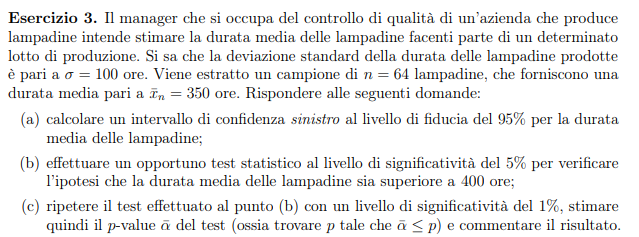
\includegraphics[width=.95\textwidth]{esami/es3_settembre23_testo.png}
\end{center}
\rispostaaperta{
	Dobbiamo stimare la media con la deviazione standard (e quindi la varianza) note. Dal formulario l'intervallo di confidenza sinistro è dato da:
	\[ (-\infty, \bar{x}_n + z_\alpha \frac{\sigma}{\sqrt{n}})\]
	Nel nostro caso abbiamo che: $n=64$, $\bar{x}_n = 350$, $\sigma = 100$. Dobbiamo trovare $z_\alpha$:
	\\ Per trovare alpha, sappiamo che $100(1-\alpha) = 95\% \implies \alpha = 5\% = 0.05$.
	\\ trovare $z_{0.05}$ significa trovare il valore di $z$ t.c. $\phi(z) = 1-\alpha = 0.95$. Dalle tavole dell distribuzione normale troviamo $z_{0.05}$ per interpolazione, infatti:
	\begin{center}
		$\phi(1.64) = 0.9495$ e $\phi(1.65) = 0.9505$, quindi $z_{0.05} = 1.645$, cioè a metà trai due.
	\end{center} 
	Sostituiamo nella fomula e troviamo che un intervallo di confidenza sinistro al 95\% per $\mu$ è:
	\[ (-\infty, 350 + 1.645 \frac{100}{8}) \simeq (-\infty, 370.56)\]
}
\rispostaaperta{
	Dobbiamo impostare un test con media incognita e varianza nota.
	Siccome ci chiediamo se $\mu > 400$, allora $H_0 : \mu \geq 400$ e $H_1 : \mu < 400$.
	\\ Dal formulario, la regione critica è $\frac{\bar{x}_n - \mu_0}{\sigma}\sqrt{n}< -z_\alpha$.
	Che significa che i dati consentono di rifiutare $H_0$ a livello di significatività $\alpha$ se questa disequazione è rispettata.
	In questo caso: $\mu_0 = 400$, $n=64$ $\bar{x}_n=350,\sigma=100,\alpha = 0.05$. Sostituendo troviamo:
	\[q<z_\alpha \to -4 < - 1.645\]
	Siccome questa disequazione è \textbf{vera} rifiuto $H_0 : \mu \geq 400$ a livello di significatività del 5\%.
	\osservazione{ Il valore 400 non appartiene all'intervallo sinistro di confidenza al 95\% per $\mu$ che abbiamo trovato nel punto precedente, quindi avremmo potuto rifiutare $H_0$ automaticamente.}
}
\rispostaaperta{
	Ripetendo il test effettuato al punto precedente ma al 1\%, troviamo $z_0.01 \simeq 2.325$ ($z$ tale che $\phi(z) = 0.9900$).
	Dato che $q$ non cambia abbiamo ancora che $-4 < - 2.325$ e quindi rifiutiamo $H_0$ al livello 1\%.

	Per il p-value del test possiamo concludere che $\bar{\alpha} \geq 0.01$ e che i dati sono in constrasto significativo con $H_0$, ovvero c'è forte evidenza statistica che la durata media delle lampadine è $< 400$ ore.

	Non stiamo a calcolare il p-value perchè dovremmo trovare un valore $\alpha$ tale per cui $z_\alpha = 4$, che sarebbe un valore estremamente piccolo, tanto che le nostre tavole vanno fino a $z_{0.0002} = 3.49$.
}
\end{document}